% 论文_问题二前两部分.tex —— 问题二前两部分(日内销售结构模型 + 七日需求预测)
% 本文件是章节片段(无 documentclass),预览请打开 论文预览.tex 编译;
% 并入主文档时作为 \input 载入,章节编号自动顺延。
% 与主文档合并时:将本文件作为 \input 载入,章节编号自动顺延;
% 图件 paper_fig1~fig5.pdf 与本文件同目录,需 \graphicspath{{p2/}} 或同目录编译;
% 定价优化部分另引用同目录 p2o2_fig_需求曲线.png、p2o3_fig1_收益曲线.png、p2o3_fig2_销售轨迹.png(png 格式)。
% 编译前须填两处表格数据(搜索 %%FILL%%)。 这个词，A检查都。
\section{问题二模型的建立与求解}

本节先刻画六品类蔬菜的日内销售结构,建立正价、品相折扣、清仓三渠道的销售模型,说明损耗率与折扣渠道的关系;再在日度尺度上建立七日需求量预测模型;最后以前两者的输出为输入,构建品类加成率的定价优化模型,给出 2023 年 7 月 1 日至 7 日的补货总量与定价策略。三者的分工是:日内结构给出各渠道的销量占比与实现价格,需求预测给出需求量及其不确定性区间,定价优化在两者之上回答收益最大化下的定价问题。

\subsection{模型假设}

\begin{enumerate}
  \item \textbf{当日售罄假设}:蔬菜类商品当日进货、当日售完,隔日无法再售。因此各日补货决策相互独立,不存在跨期库存结转。
  \item \textbf{折扣档位假设}:折扣销售存在两个稳定档位,19 时前为品相折扣档(折后价约为原价的 0.80~0.91),19 时起为清仓档(多数品类折后价为原价的 0.600);茄类例外,全天约 0.83 档。渠道归属一律以 19 时为界。
  \item \textbf{损耗口径假设}:附件 4 的损耗率 $\theta$ 为近期盘点口径,刻画进货与陈列中的商品损耗;按题面机制,运损与品相变差的商品通常经折扣渠道售出,故损耗商品与折扣渠道相对应。$\theta$ 同时用作补货换算参数,即补货总量 $=$ 需求$/ (1-\theta)$。
  \item \textbf{需求口径假设}:品类日需求量取正价、品相折扣、清仓三渠道销量合计。疑似提前售罄日的观测销量只构成需求的下界,训练与评价中按删失数据处理。
  \item \textbf{日历假设}:节假日效应以春节、国庆、五一的法定假期窗口哑变量刻画;星期效应用星期哑变量与周季节分解刻画。不考虑天气、客流量、竞争价格等附件未提供的外生变量,其影响并入残差,由分位数区间覆盖。
  \item \textbf{定价机制假设}:加成率 $\kappa$ 每品类每日取一个值,挂牌价 $=$ 当日成本 $\times (1+\kappa)$;日内折扣档位及其 19 时的触发时刻是门店的固定政策,不随 $\kappa$ 变化,$\kappa$ 只平移价格水平。
\end{enumerate}

其中假设 3 与假设 4 需要说明设计理由。假设 3 将损耗率与折扣渠道对应起来:一是承接题面"对运损和品相变差的商品通常进行打折销售"的机制,使折扣渠道的构成有明确的物理含义;二是使收益核算互洽,折扣渠道进入收入端、$\theta$ 进入补货的成本端,若两者脱钩,收益模型会同时漏掉损耗成本与折扣收入。附件 4 的 $\theta$ 是近期盘点口径,与附件 2 三年流水的统计窗口不同,本文因此只把 $\theta$ 用作渠道机制与补货换算的参数,折扣渠道的日内与品类结构则由附件 2 实测给出。假设 4 若不成立,即把售罄日的低销量当作真实需求,滞后特征将被系统性污染:例如某日 15 时即售罄、记录销量 120 kg,而真实需求约 150 kg,模型会把该日当低需求日学习,进而低估未来一周的需求。假设 4 的具体处理见 \ref{subsec:censor}。假设 6 是价格响应可识别的前提:若门店执行随剩余库存调整折价深度的保售罄规则,折扣与定价互为因果,加成率的效应无法从历史数据中分离;把折价档位固定为政策之后,加成率的作用集中在挂牌价水平上,才能与成本冲击分离开。

\subsection{日内销售结构模型}

\subsubsection{渠道划分与损耗率的关系}

对 2020 年 7 月 1 日至 2023 年 6 月 30 日共 878{,}042 条销售流水(已剔除退货),我们按时段$\times$是否打折把每条记录划入三个渠道:不打折记为正价渠道;19 时前打折记为品相折扣渠道,对应题面所述运损与品相受损但仍可售的商品;19 时起打折记为清仓渠道,对应日终未售完商品的降价出清。这样划分的依据是折扣深度的时间结构:全部品类 19 时前的折后价位于原价的 0.80~0.91 档,19 时后多数品类精确落在 0.600 档,呈两档式政策结构,而非随时间连续衰减,故以 19 时为界切分。

在该口径下,损耗率 $\theta$ 与品相折扣渠道相对应:运损与品相变差的商品经折扣渠道变现,清仓渠道则承接当日未售完的部分。表 \ref{tab:theta} 列出各品类的近期损耗率,它在后文的收益模型中进入补货成本端。

\begin{table}[htbp]
  \centering
  \caption{各品类近期损耗率 $\theta$(附件 4)}
  \label{tab:theta}
  \begin{tabular}{lcccccc}
    \toprule
    品类 & 花叶类 & 食用菌 & 辣椒类 & 水生根茎类 & 茄类 & 花菜类 \\
    \midrule
    $\theta$/\% & 12.83 & 9.45 & 9.24 & 13.65 & 6.68 & 15.51 \\
    \bottomrule
  \end{tabular}
\end{table}

\subsubsection{日内销量分布与渠道结构}

图 \ref{fig:intraday} 给出水生根茎类的日内销量结构(占该品类全期销量的百分比)。销量呈三段式:9 至 10 时为开店高峰,16 至 18 时为次高峰,19 时起进入清仓时段。单小时峰值出现在 10 时,约 18\%;清仓渠道的销量集中在 19 至 21 时,品相折扣则零散分布在 9 至 18 时之间。

\begin{figure}[htbp]
  \centering
  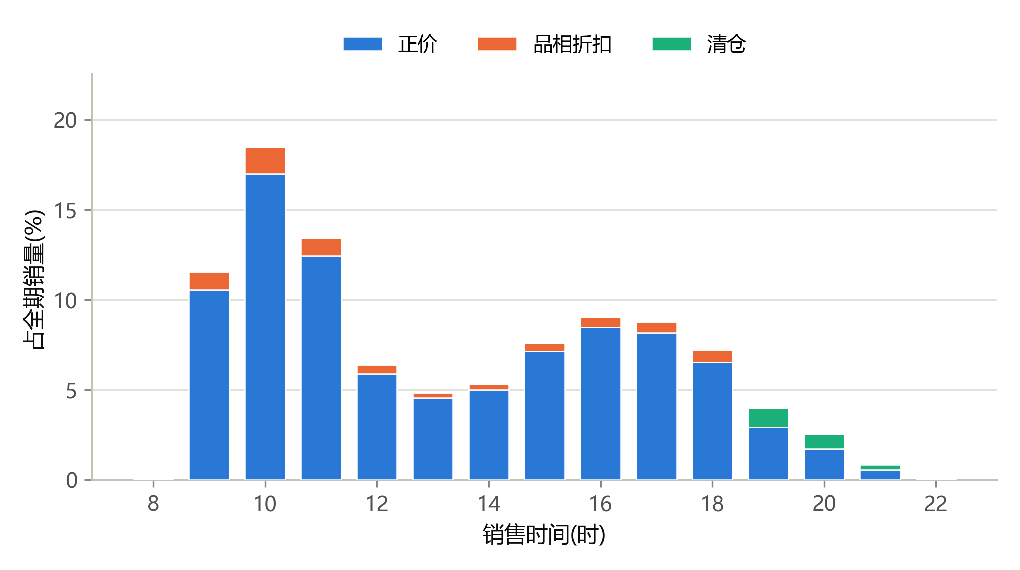
\includegraphics[width=0.92\textwidth]{paper_fig1.pdf}
  \caption{水生根茎类日内销量结构(占全期销量比重/\%,按渠道堆叠)}
  \label{fig:intraday}
\end{figure}

图 \ref{fig:channel} 汇总六品类的渠道构成。正价渠道占各品类销量的 91.0\%~97.3\%,是绝对主体。品相折扣渠道的占比存在品类差异:水生根茎类最高,为 6.9\%,花叶类与茄类最低,约 2.0\%。清仓渠道的分化更明显,食用菌为 5.4\%、花叶类为 4.7\%,茄类仅 0.68\%。以清仓与品相折扣的销量之比衡量两类渠道的相对强度,花叶类为 2.35、食用菌为 1.88,呈清仓主导型;水生根茎类为 0.31、茄类为 0.34,呈品相主导型。这一差异与其货架期和损耗特性一致:叶菜类当日未售出的余量大、清仓需求强,茄类耐存放、折扣以挑拣产生的品相损失为主。

\begin{figure}[htbp]
  \centering
  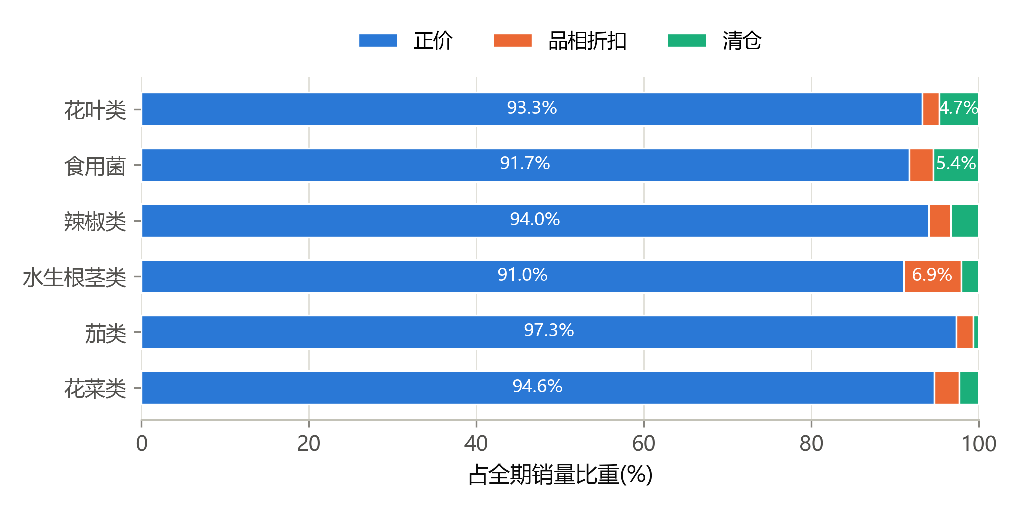
\includegraphics[width=0.92\textwidth]{paper_fig2.pdf}
  \caption{六品类渠道结构(占全期销量比重/\%)}
  \label{fig:channel}
\end{figure}

\subsubsection{折扣深度的时间结构}

花叶类打折记录的折后价与原价之比(中位)在日间从 9 时的 0.81 单调降至 18 时的 0.69(图 \ref{fig:depth}),反映商品随陈列时间增加而品相变差、折价逐步加深;19 时起跳变至 0.600 档并保持稳定,对应定时清仓政策。这条曲线同时给出了分时段定价所需的折扣深度函数,也是 19 时渠道划分依据的直接证据。

\begin{figure}[htbp]
  \centering
  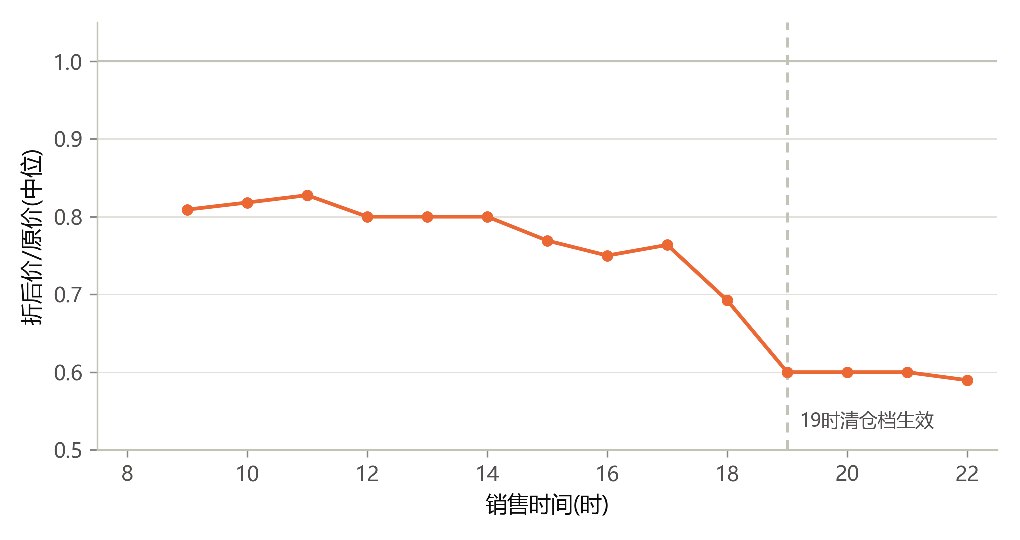
\includegraphics[width=0.92\textwidth]{paper_fig3.pdf}
  \caption{花叶类日内折扣深度曲线(折后价/原价中位,1.0 为原价)}
  \label{fig:depth}
\end{figure}

\subsection{基于周季节分解与 LightGBM 分位数回归的七日需求预测}

\subsubsection{建模思路}

需求预测有三件事要先界定,即预测对象、周季节与节假日的剥离方式,以及销量不等于需求时的处理。预测对象定为三渠道销量合计的品类日需求量,与补货总量的口径一致;周季节由经典加法分解剥离,节假日与月份作为特征交由模型学习;销量对需求的截断则通过一个数据驱动的售罄检测器显式处理,这是本模型与常规做法的主要差别。

\subsubsection{周季节分解}

设品类日销量为 $Q_t$,取 $y_t=\ln(Q_t+0.1)$ 进入模型。周季节采用经典加法分解:
\begin{equation}
  y_t = T_t + S_{w(t)} + \varepsilon_t,
\end{equation}
其中 $T_t$ 为 7 日滑动平均趋势项,$w(t)$ 为 $t$ 日的星期序号,季节因子
\begin{equation}
  S_w = \operatorname*{median}_{t:\,w(t)=w,\,Q_t>0}\,\left(y_t - T_t\right),
\end{equation}
模型在去季节序列 $\tilde{y}_t = y_t - S_{w(t)}$ 上训练,预测时加回 $S_{w(t)}$。分解所需统计量只在各折训练窗内估计;训练窗最后 3 天的趋势项强制用 trailing 窗口计算,避免居中窗口引用未来数据。

\subsubsection{提前售罄检测与删失处理}
\label{subsec:censor}

销量是需求被库存截断后的实现值,售罄日的观测销量低估真实需求,而附件并未提供缺货记录。为此我们构造了一个只依赖销售流水的提前售罄检测器:记品类第 $t$ 日最后一次成交时刻为 $L_t$(时),若
\begin{equation}
  L_t \le \operatorname*{median}\left\{L_{s}:\, s \text{ 为 } t \text{ 前 8 个同星期日}\right\} - 3
  \quad\text{且}\quad
  Q_t \ge \tfrac{1}{2}\,\operatorname*{median}\{Q_{t-28},\dots,Q_{t-1}\},
  \label{eq:censor}
\end{equation}
则将第 $t$ 日标记为疑似提前售罄日。其含义是:营业时长与近期同星期几基本一致,打烊时刻却大幅提前且销量并不偏低,说穿了,就是下午把货卖空了。全部 6 品类 6570 个品类日中共检出 62 天,占比 0.9\%,其中水生根茎类 23 天、茄类 22 天、花菜类 14 天、食用菌 3 天,花叶类与辣椒类为 0 天;检出集中于销量小、波动大的品类,与其断货机理相符。

检测结果在模型中有三处用途。其一作为特征,售罄标记的滞后值(滞后 7 天与近 7 天检出频率)进入特征矩阵,使模型得以甄别滞后项中被截断的低值。其二作为训练样本处理,保守方案将标记日从训练中剔除,不以其有偏观测参与拟合,进一步地,利用任务一日内销售结构模型给出的累计销量曲线,把截断日的观测销量按其打烊时刻放大到全天水平,作为需求估计参与训练,记为修复方案。其三作为评价口径,回测指标分全样本与剔除疑似售罄日两套报告。三种处理连同不作处理的对照一起,由 \ref{subsec:bt} 的消融实验择优。

\subsubsection{LightGBM 分位数回归与直接多步设计}

六个品类共 6570 个日度观测合并为一个训练集,品类以哑变量进入。模型为 LightGBM 分位数回归,目标取 $\alpha=0.1,0.5,0.9$ 三个分位数的分位损失,树数 400、学习率 0.05、叶子数 31、叶最小样本数 30,其余取默认值。这一选型有方法学与领域文献两方面的依据。方法上,梯度提升树自 Ke 等提出 LightGBM 以来\cite{ke2017},凭对非线性关系与特征交互的高效刻画成为表格数据预测任务的主力;Grinsztajn 等在中等规模表格数据集上的系统比较进一步表明,树模型的整体表现仍优于深度网络\cite{grinsztajn2022}。领域上,零售需求预测的近期文献结论一致:Lyulyov 对某连锁超市 13 种预测方法的比较中,调参后的 LightGBM 取得最低误差\cite{lyulyov2024};Fan 等针对生鲜品类快速响应供应链构建的 LightGBM 混合模型,也报告了优于对照方法的预测精度\cite{fan2024}。相比之下,单序列深度模型在中小规模序列上并无稳定的优势证据,故本文不引入此类模型。目标变量为去季节后的 $\tilde{y}_t$,预测值经 $\hat{Q}_\alpha=\exp(\hat{q}_\alpha)-0.1$ 换算回千克;由于单调变换保持分位数,该换算是精确的,且保证预测非负。

特征共 37 维,分四组。滞后组是 $\tilde{y}$ 的 7、14、21、28 日滞后及其平移 7 日的 28 日滚动均值与标准差,断货组是式 (\ref{eq:censor}) 标记的滞后值,日历组含星期、月份、年份哑变量与节假日标记,品类组为品类哑变量。滞后项全部取 7 天及更早,单个模型因而能直接输出未来 7 天的预测,不依赖递归调用,避免多步递归的误差累积。

\subsubsection{基线模型与回测方案}
\label{subsec:bt}

设两条基线。季节朴素基线取 $\hat{Q}_t = Q_{t-7}$,即直接以上周同日销量作为预测,它是时序预测的标准下界参照。统计基线取岭回归,与主模型共用同一套周季节分解和特征矩阵,只在模型层以线性回归替代梯度提升树,用以分离特征工程与非线性模型各自的贡献。

回测采用滚动起点方案:自 2023 年 1 月 2 日起每周一个起点,共 24 折,每折以起点前全部数据训练、预测其后 7 天,覆盖 2023 年上半年。评价指标中,加权绝对百分比误差
\begin{equation}
  \mathrm{WAPE}=\frac{\sum_t \left|Q_t-\hat{Q}_t\right|}{\sum_t Q_t},
\end{equation}
直接给出相对总量的误差水平;MASE 与 RMSSE 分别以训练窗内季节差分的平均绝对值和均方根为标尺,
\begin{equation}
  \mathrm{MASE}=\frac{\operatorname*{mean}\left|Q_t-\hat{Q}_t\right|}
  {\operatorname*{mean}\left|Q_t-Q_{t-7}\right|},
  \qquad
  \mathrm{RMSSE}=\frac{\sqrt{\operatorname*{mean}\left(Q_t-\hat{Q}_t\right)^2}}
  {\sqrt{\operatorname*{mean}\left(Q_t-Q_{t-7}\right)^2}},
\end{equation}
两者小于 1 即优于季节朴素基线;分位数质量以 pinball 损失评价,
\begin{equation}
  L_\alpha(y,\hat{q})=\operatorname*{mean}\left[\alpha\,(y-\hat{q})\,\mathbf{1}_{y\ge\hat{q}}+(1-\alpha)\,(\hat{q}-y)\,\mathbf{1}_{y<\hat{q}}\right].
\end{equation}

\begin{table}[htbp]
  \centering
  \caption{回测指标对照(2023 年 24 折滚动平均)}
  \label{tab:bt}
  \begin{tabular}{lcccccc}
    \toprule
    模型 & WAPE & MASE & RMSSE & pinball10 & pinball50 & pinball90 \\
    \midrule
    STL+LightGBM(断货修复) & 0.2406 & 0.730 & 0.516 & 3.95 & 9.18 & 6.55 \\
    STL+LightGBM(断货剔除) & 0.2440 & 0.734 & 0.520 & 3.92 & 9.17 & 6.64 \\
    STL+LightGBM(无断货处理) & 0.2447 & 0.741 & 0.525 & 3.95 & 9.33 & 6.47 \\
    STL+岭回归 & 0.2874 & 0.834 & 0.580 & -- & -- & -- \\
    季节朴素 & 0.3060 & 0.929 & 0.660 & -- & -- & -- \\
    \bottomrule
  \end{tabular}
\end{table}

表 \ref{tab:bt} 与图 \ref{fig:wape} 给出回测结果。主模型 STL+LightGBM(断货修复)的整体 WAPE 为 0.2406,比不作断货处理的同型模型降低 1.7\%,比岭回归基线降低 16.3\%,比季节朴素基线降低 21.4\%;MASE 为 0.730,小于 1,7 天预测误差比直接照抄上周同日低 27.0\%。消融实验中两档断货处理均优于不作处理,且修复档最优,说明任务一的日内结构不仅刻画了销售形态,其累计销量曲线反哺训练目标后还带来了额外收益。分品类来看,修复档在六个品类全部持平或占优,改善最大的为茄类(WAPE 由 0.288 降至 0.281)与花叶类、食用菌(约降 2.6\%);花叶类与辣椒类全期未检出售罄日,各档结果几乎重合,该处理对它们没有副作用。图 \ref{fig:wape} 左下还显示,主模型在全部六个品类上的 WAPE 均低于两条基线,误差最大的为水生根茎类(0.295),最小的为花叶类(0.180)。

\begin{figure}[H]
  \centering
  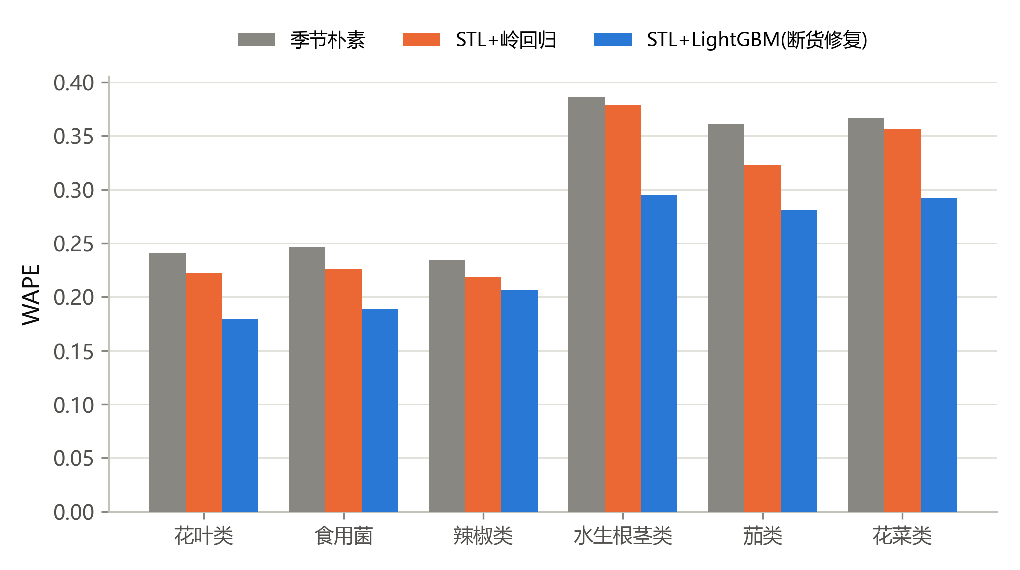
\includegraphics[width=0.92\textwidth]{paper_fig5.pdf}
  \caption{分品类 WAPE 对照:主模型与两条基线(24 折滚动平均)}
  \label{fig:wape}
\end{figure}

\subsubsection{七日需求量预测结果}

按消融结论,最终模型采用断货修复处理、以全部历史重训,输出 2023 年 7 月 1 日至 7 日六品类的日需求量 P10、P50、P90。表 \ref{tab:fc} 给出 P50 中位预测。

\begin{table}[htbp]
  \centering
  \caption{2023 年 7 月 1 日至 7 日六品类日需求量 P50 预测(kg/日)}
  \label{tab:fc}
  \begin{tabular}{lcccccc}
    \toprule
    日期 & 花叶类 & 食用菌 & 辣椒类 & 水生根茎类 & 茄类 & 花菜类 \\
    \midrule
    7 月 1 日 & 204.6 & 67.6 & 107.2 & 26.9 & 32.0 & 34.5 \\
    7 月 2 日 & 169.7 & 59.9 & 85.0 & 26.5 & 34.4 & 29.8 \\
    7 月 3 日 & 130.9 & 42.5 & 75.6 & 15.1 & 23.2 & 19.7 \\
    7 月 4 日 & 149.0 & 43.1 & 71.3 & 18.5 & 16.6 & 20.4 \\
    7 月 5 日 & 154.7 & 52.2 & 69.3 & 20.9 & 20.1 & 23.6 \\
    7 月 6 日 & 150.9 & 49.8 & 79.4 & 28.9 & 18.1 & 24.8 \\
    7 月 7 日 & 152.2 & 55.8 & 77.5 & 23.5 & 23.4 & 28.5 \\
    \bottomrule
  \end{tabular}
\end{table}

图 \ref{fig:fc} 以花叶类为例给出预测与近期历史的对照。7 月 1 日(周六)的预测为 204.6 kg,明显高于 6 月 30 日(周五)的 130.5 kg。我们专门核查了这一跳变:花叶类 6 月 30 日售满全天(最后成交时刻 21 时,与近 8 个同星期日的中位一致),未触发式 (\ref{eq:censor}) 的售罄标记,故就花叶类自身而言,该跳变不宜归因于断货,来源是星期效应,花叶类近三年周六平均销量 229.3 kg,为全周最高,约为周一至周四均值的 1.4 倍,预测值恰好落在近期周六 161.5~244.3 kg 的区间之内。同时,预测窗前其他品类检出的提前售罄日(如花菜类 6 月 18 日)对应的被截断需求,已经由修复处理回补进训练目标,构成 7 月初需求水平上浮的次要因素。P10 至 P90 区间在周末与销量较大的品类上更宽,区间宽窄就是补货余量的选择空间,按 P50 补货约半数日子会缺货,按 P90 补货仅约一成日子缺货,但积压风险随之上升;两者如何取舍,交由下文的定价优化模型结合缺货与积压损耗成本确定。

\begin{figure}[H]
  \centering
  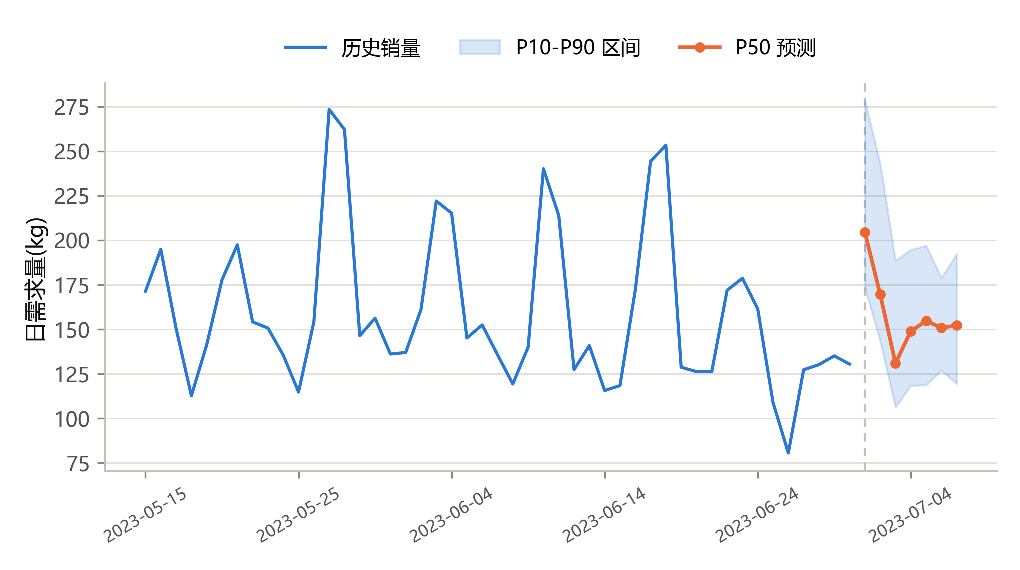
\includegraphics[width=0.92\textwidth]{paper_fig4.pdf}
  \caption{花叶类日需求量预测(2023 年 7 月 1 日至 7 日,近 45 天历史与 P10 至 P90 区间)}
  \label{fig:fc}
\end{figure}

\subsection{基于半对数需求响应与期望收益的品类定价优化}
\label{subsec:pricing}

\subsubsection{补货量界定与决策变量}

上一小节给出了七日需求量的中位预测与分位区间,本节在其之上回答定价问题。按假设 1 与假设 3,第 $c$ 品类第 $d$ 日的补货总量取
\begin{equation}
  Q_{c,d}=\hat{Q}^{P50}_{c,d}/(1-\theta_c),
\end{equation}
即按中位预测备货、再按损耗率补足报废部分。补货量外生固定,决策变量只有加成率 $\kappa_{c,d}$,挂牌价为 $P_{c,d}=\hat{c}_c\,(1+\kappa_{c,d})$,其中 $\hat{c}_c$ 为近 8 周销量加权平均批发价。为什么不把补货量与加成率放在一起联合寻优?加成率提高时,同样的补货量必然卖不完,售罄率是模型的内生结果而不是约束条件,把它交给逐窗清算机制处理即可;联合优化只是把同一笔账换个记法,却多出一层寻优与一组一致性约束。

\subsubsection{半对数需求响应的构建}
\label{subsec:resp}

定价优化的核心输入是需求对价格的响应。我们的做法分三步:先定形式,再解决识别,最后修正删失。

形式上取半对数
\begin{equation}
  \ln Q^{(c)}_t=\alpha_c-b_c P^{(c)}_t+\gamma^{\top}X_t+\varepsilon_t,
  \label{eq:semilog}
\end{equation}
其中 $Q^{(c)}_t$ 为品类日需求量,$P^{(c)}_t$ 为当日正价销量加权均价,$X_t$ 含年月与星期固定效应。不用更常见的对数线性(等弹性)形式,原因有二。其一,等弹性需求在弹性小于 1 时收益关于价格单调递增,最优解永远顶在价格可行域边缘,这是收益管理文献中的标准结论\cite{phillips2005};其二,对数形式的需求随价格指数发散,向历史观测域之外外推没有边界。半对数形式下收益函数 $\pi(P)=P\exp(\alpha-bP)$ 在 $P^{\ast}=1/b$ 处取得内点最大,需求随价格升高有界趋于零,天然具备这两条性质。同时,Besbes 与 Zeevi 证明,即使真实需求是非参数的,以简单参数形式在历史价格域内寻优也已近乎最优\cite{besbes2015},这为后文把搜索限制在历史价域内的做法提供了理论依据。

识别上不能直接做最小二乘。我们先做了一步对照:对 2020 年 7 月至 2023 年 6 月的品类日度面板直接回归,价格系数为正,六品类隐含弹性高达 $+2.2$ 至 $+6.6$,字面意思是"越贵卖得越多",显然是混杂而非因果:批发成本上涨的日子零售价随之走高,需求旺盛的日子门店也顺势标高价,价格与销量被同一批因素同向推动。因此取批发价对数作工具变量做两阶段最小二乘:批发价由上游批发市场决定,不影响门店客流,它作用于销量的唯一通道是迫使零售价变动。一阶段 $F$ 统计量为 1698~4564,远超弱工具变量的警戒线;标准误按 Newey-West 异自相关一致估计计算,滞后取 21 日,以吸收日度销量的序列相关。

删失修正沿用断货时点信息的思路\cite{jain2015}。销量是需求被库存截断后的实现值,直接回归会把价格响应向零压低。这里的检测器与预测小节的售罄检测器(式 \ref{eq:censor})取向不同:预测处的检测器要求精确,宁漏勿误,检出 0.9\%;此处的检测器要求召回,当日 19 时后的销量份额低于该品类分布的 10\% 分位即判定为提前售罄,六品类检出率约 10\%(水生根茎类为 0)。对判定为删失的日期,观测销量就是库存上限,真实需求只知不小于它,用变上限删失回归的 EM 算法补全:
\begin{equation}
  E\!\left[\ln Q\,\middle|\,\ln Q>\ln S\right]
  =x^{\top}\beta+\sigma\,\frac{\varphi(z)}{1-\Phi(z)},
  \qquad z=\frac{\ln S-x^{\top}\beta}{\sigma},
  \label{eq:em}
\end{equation}
其中 $S$ 为当日观测销量,$\varphi$ 与 $\Phi$ 为标准正态密度与分布函数。EM 收敛后,以补全需求 $Q^{\mathrm{adj}}$ 重估式 (\ref{eq:semilog}),价格系数仍由两阶段最小二乘给出。

\subsubsection{估计结果与文献先验收缩}
\label{subsec:eb}

表 \ref{tab:elas} 汇总六品类的估计结果。主估计的价格系数落在 0.012~0.045,全部在 5\% 水平显著,隐含弹性(弹性等于 $-b\bar{P}$,$\bar{P}$ 为近期均价)在 $-0.12$ 至 $-0.40$ 之间。对照列给出三组参照:不做删失修正的估计、DML-PLIV 对照\cite{chernozhukov2018}(五折交叉拟合,梯度提升树拟合多余函数)与 Laspeyres 固定权重口径。三点解读。其一,删失修正几乎没有移动系数(如花叶类 0.063 对 0.045),10\% 的删失率不足以解释弹性偏低,压低响应的主因不在删失。其二,DML 口径给出的响应强一个量级,但品类间离散过大,水生根茎类的隐含弹性达到 $-6$,在千余观测的小样本上不可尽信。其三,Laspeyres 口径的系数连符号都不稳定,从反面印证销量加权均价确实被单品构成变化污染,这是品类级数据自带的局限。

\begin{table}[htbp]
  \centering
  \caption{需求响应估计:半对数系数 $b$ 的多口径对照(2020-07 至 2023-06,日度)}
  \label{tab:elas}
  \begin{tabular}{lccccccc}
    \toprule
    品类 & 不修正 & 主估计 & HAC se & DML-PLIV & 后验收缩 & 隐含弹性 & 近期均价/元 \\
    \midrule
    花叶类 & 0.063 & 0.045 & 0.007 & 0.328 & 0.047 & $-0.26$ & 5.60 \\
    食用菌 & 0.025 & 0.016 & 0.006 & 0.337 & 0.018 & $-0.15$ & 8.23 \\
    辣椒类 & 0.017 & 0.012 & 0.006 & 0.237 & 0.014 & $-0.12$ & 8.43 \\
    水生根茎类 & 0.033 & 0.033 & 0.009 & 0.416 & 0.035 & $-0.31$ & 8.72 \\
    茄类 & 0.018 & 0.023 & 0.012 & 0.163 & 0.029 & $-0.25$ & 8.56 \\
    花菜类 & 0.045 & 0.044 & 0.007 & 0.936 & 0.045 & $-0.41$ & 9.16 \\
    \bottomrule
  \end{tabular}
\end{table}

对食品价格弹性的系统综述显示,多数食品品类的弹性绝对值介于 0.3 与 0.8 之间,蔬菜水果类居于其中偏高的位置\cite{andreyeva2010}。我们的主估计比这一区间还要靠下不少,数据与文献谁对?我们不做非此即彼的取舍,而是按经验贝叶斯把文献区间设为先验、数据似然作证据,按方差倒数加权收缩:
\begin{equation}
  b^{\mathrm{post}}_c=\frac{\hat{b}_c/\sigma^2_c+b_{0,c}/\tau^2_{0,c}}
  {1/\sigma^2_c+1/\tau^2_{0,c}},
  \label{eq:eb}
\end{equation}
先验中枢取 $b_{0,c}=0.7/\bar{P}_c$(对应弹性 $-0.7$)、标准差 $\tau_{0,c}=0.3/\bar{P}_c$,覆盖文献主要区间。收缩的结果出乎直觉,但信息量更大:数据权重达 90\%~98\%,后验几乎完全跟随数据。换成假设检验的语言,本店数据以最少约 4 个、至多约 12 个标准差的幅度拒绝了文献先验,该商超顾客的价格敏感度确实远低于文献水平。可能的原因有三:单店品类级数据缺乏替代品竞争的变异;社区客群相对固定;样本期内没有促销干预。图 \ref{fig:demand} 给出收缩前后的需求曲线,数据口径与后验口径在历史价域内几乎重合,虚线对照则显示出删失偏差被纠正的幅度。

\begin{figure}[htbp]
  \centering
  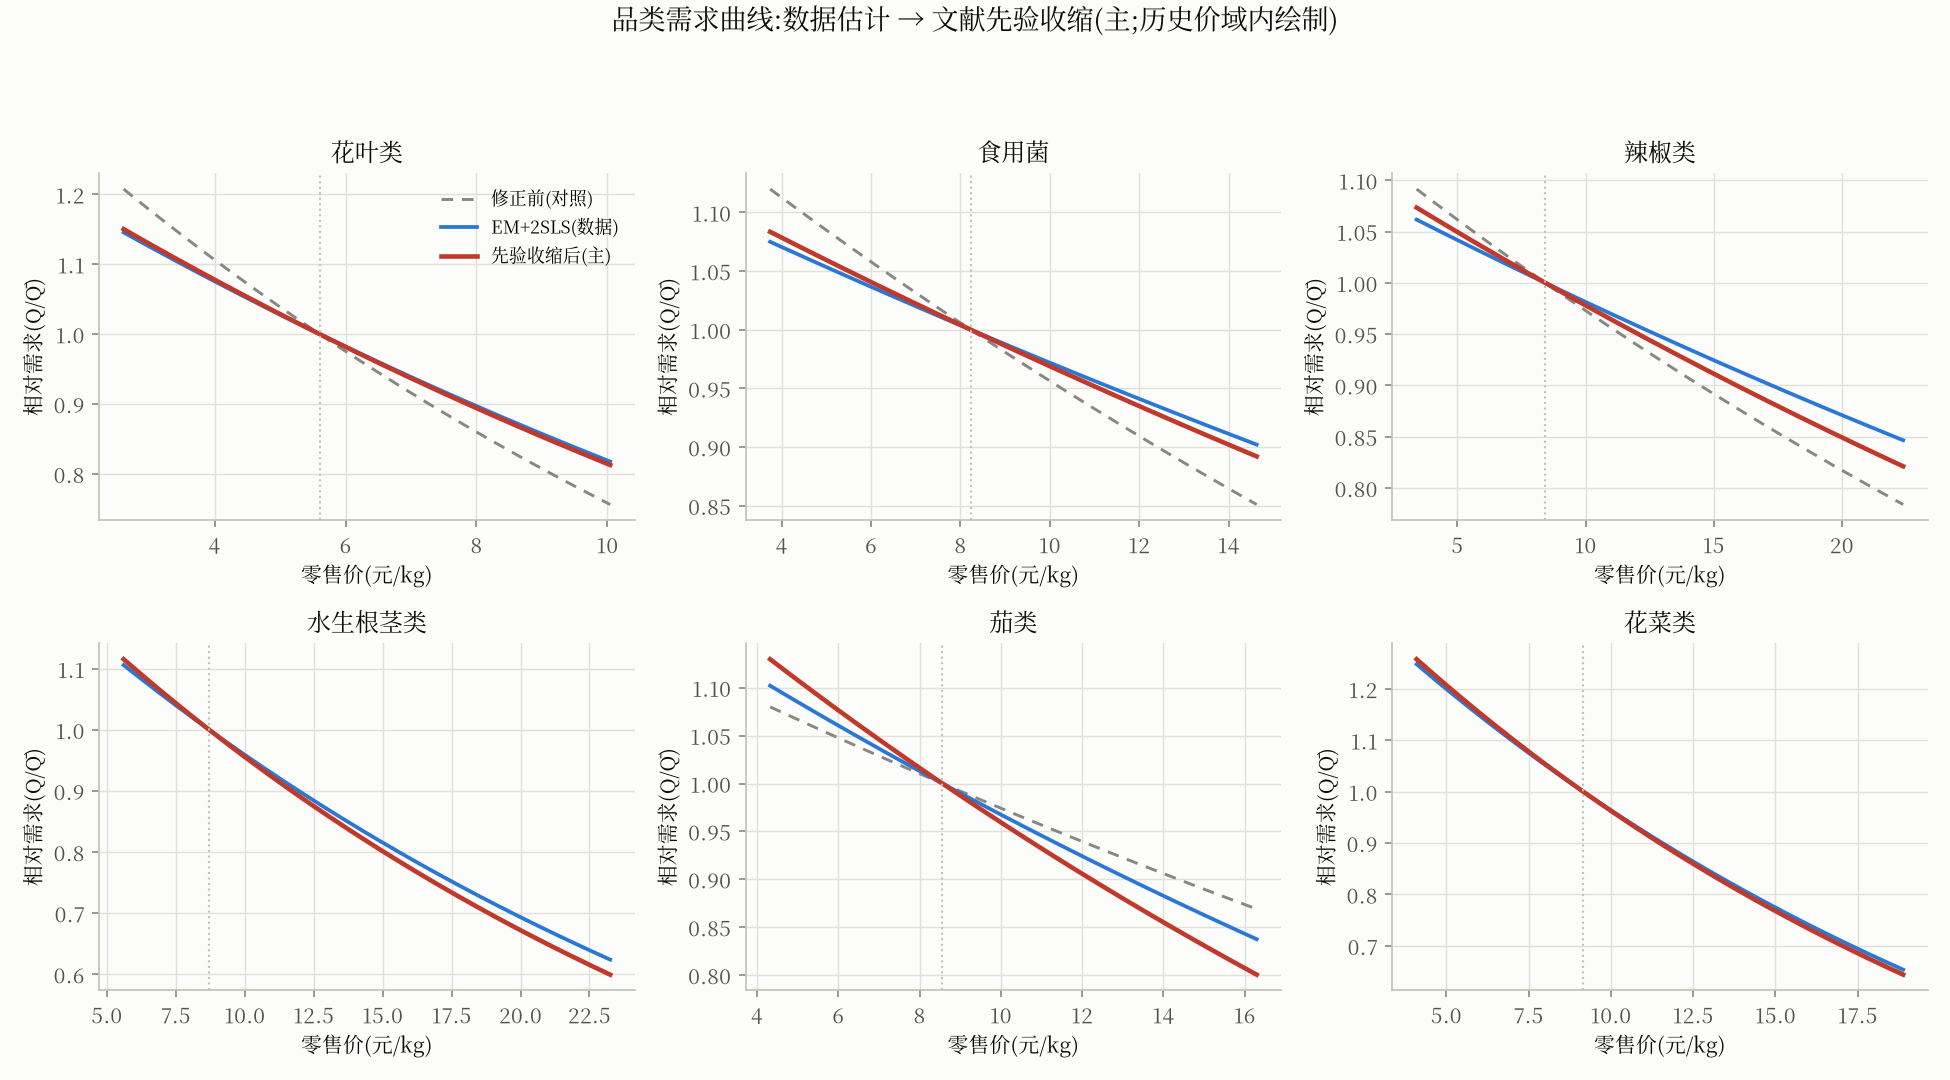
\includegraphics[width=0.92\textwidth]{p2o2_fig_需求曲线.png}
  \caption{六品类需求曲线:数据估计与文献先验收缩(历史价域内,相对近期均价)}
  \label{fig:demand}
\end{figure}

按后验弹性,半对数需求的无约束最优价为 $1/b^{\mathrm{post}}$,六品类落在 21.1~70.9 元/kg,全部高出历史价域上缘一倍以上。响应微弱叠加信任域约束,定价寻优呈现角点解形态,这在下文的结果中还会出现。

\subsubsection{期望收益模型}

收益模型把预测分位、日内结构与价格响应拼在一起。日需求量做对数正态抽样,对数标准差由预测分位距换算,$\sigma_d=(\ln P90-\ln P10)/(2\times1.2816)$。营业日按小时切窗,窗口份额 $\bar{w}_t$ 与窗口实现价比 $\rho_t$ 取自旺季(4 至 10 月)实测:正价主导的白天 $\rho_t\approx1$,19 时起进入清仓档,$\rho_t$ 约 0.9。给定加成率 $\kappa$,挂牌价 $P=\hat{c}(1+\kappa)$,需求期望 $D=N^{50}\exp(-b^{\mathrm{post}}(P-\bar{P}))$,库存从 $I_9=N^{50}$ 起逐窗清算:
\begin{equation}
  s_t=\min\left(D\,\bar{w}_t\,m,\; I_t\right),\qquad I_{t+1}=I_t-s_t,
  \label{eq:clear}
\end{equation}
其中 $m$ 为对数正态需求乘数。当日收益与其期望为
\begin{equation}
  \Pi(\kappa)=E_{m}\!\left[\sum_{t=9}^{22}P\,\rho_t\,s_t\right]
  -\frac{\hat{c}\,N^{50}}{1-\theta}.
  \label{eq:profit}
\end{equation}
收档剩余计零残值:高加成率的代价不是折扣打得更深,而是卖不完的货全额损失;低加成率则早早售罄,晚间清仓时段反而无货可折。清仓悬崖由此内生化,而不再是一条外生假设。

\subsubsection{求解算法}

决策变量是一维的,目标关于加成率分段光滑,求解用 201 点稠密网格加黄金分割细化:网格保证全局性,细化把精度提到任意水平,单个品类日只需数百次浮点评估,42 个问题毫秒级出齐。没有使用整数规划类求解器,那需要把逐窗取小运算做大 M 线性化、把响应函数砍成分段线性,为用求解器而给模型加假设,得不偿失。价格搜索限制在历史价域(各品类日均价的 0.5\% 与 99.5\% 分位)之内:响应模型只在域内可信,信任域同时是外推保护。

\subsection{定价结果与策略分析}

\subsubsection{七日定价结果}

全渠道 42 个品类日的最优解全部落在信任域上缘,周期望收益 17141 元,比维持现价多 13095 元。表 \ref{tab:price} 给出分品类汇总。

\begin{table}[htbp]
  \centering
  \caption{2023 年 7 月 1 日至 7 日分品类定价结果(信任域=历史零售价域)}
  \label{tab:price}
  \begin{tabular}{lcccccc}
    \toprule
    品类 & 周补货量/kg & $\kappa^{\ast}$ & 挂牌价/(元/kg) & 期望售罄率 & 周期望收益/元 & 周增益/元 \\
    \midrule
    花叶类 & 1275.7 & 1.95 & 10.04 & 0.80 & 4393 & 3081 \\
    食用菌 & 409.6 & 3.24 & 14.63 & 0.86 & 3076 & 1774 \\
    辣椒类 & 623.0 & 5.03 & 22.39 & 0.81 & 7765 & 5725 \\
    水生根茎类 & 185.7 & 1.30 & 23.25 & 0.59 & 316 & 987 \\
    茄类 & 179.9 & 2.39 & 16.29 & 0.77 & 1217 & 818 \\
    花菜类 & 214.5 & 1.30 & 18.88 & 0.63 & 374 & 710 \\
    \bottomrule
  \end{tabular}
\end{table}

图 \ref{fig:profit} 给出收益关于加成率的完整曲线。六品类曲线在域内整体上行,水生根茎类与花菜类在后半段明显趋平,是仅有的两条出现弯折的曲线;维持现价 $\bar{\kappa}$(竖虚线)处两类品类的收益为负,提价首先把亏损定价拉回成本线之上。角点解的含义需要说清楚:模型并不认为加成率越高越好,而是在数据支撑的价格域内收益单调上升;域缘对应的历史高价包含供给冲击日的成分,机械照搬到执行层并不合适,我们据此给出的建议是温和上调并监测,这层意思在灵敏度小节展开。

\begin{figure}[htbp]
  \centering
  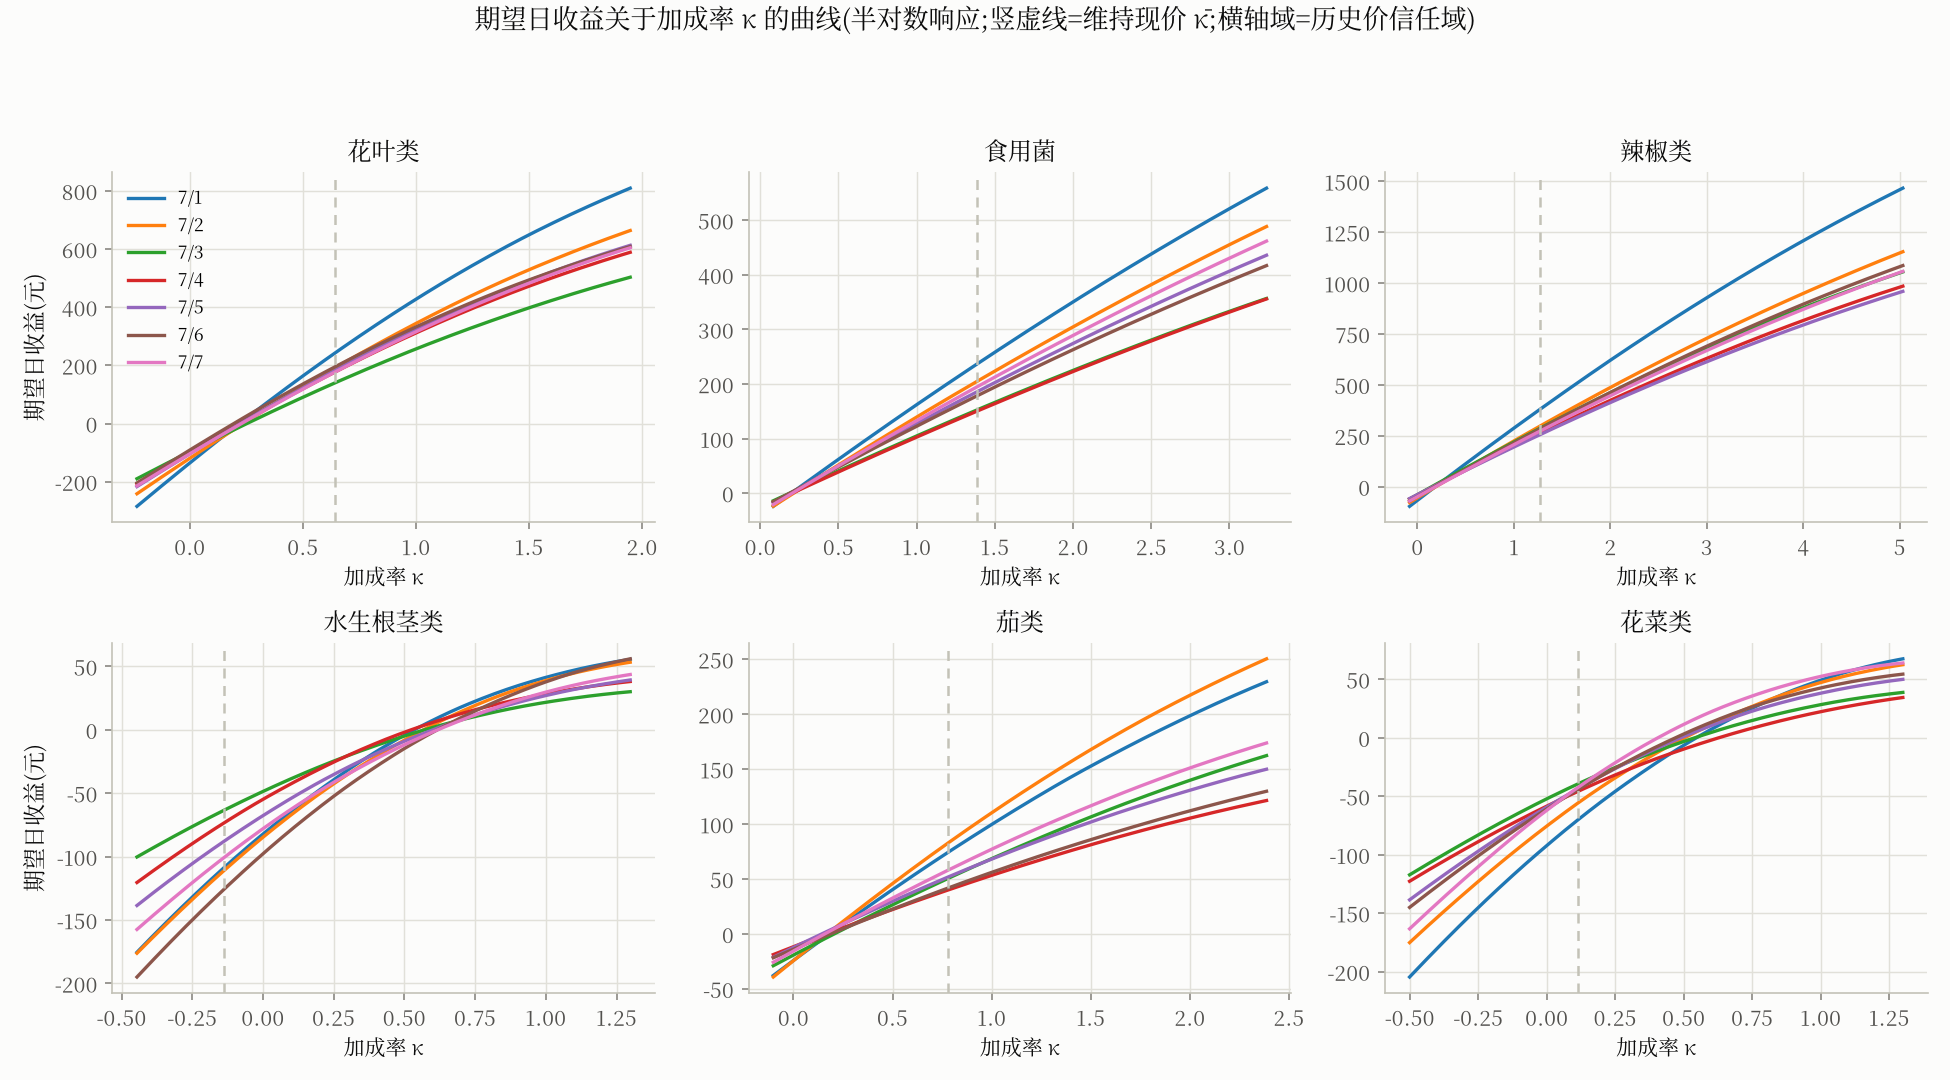
\includegraphics[width=0.92\textwidth]{p2o3_fig1_收益曲线.png}
  \caption{期望日收益关于加成率 $\kappa$ 的曲线(竖虚线为维持现价,横轴范围即历史价信任域)}
  \label{fig:profit}
\end{figure}

\subsubsection{亏损品类的定价修复}

水生根茎类与花菜类维持现价是亏本的。前者近 8 周批发均价 10.12 元/kg,已高于历史均价口径下的现价 8.72 元,每卖 1 kg 倒贴约 1.4 元;后者现价虽有约 12\% 的加成,但期望售罄率只有六成,按损耗率换算的补货量卖不完,报废吃掉了全部毛利。这笔账是算得清的:提价后水生根茎类售罄率降至 0.59,但单价跨过成本线,周增益 987 元;花菜类售罄率 0.63,周增益 710 元。图 \ref{fig:traj} 以花叶类为例对比了最优加成率与维持现价两种方案下的日内销售轨迹,提价方案的需求整体收缩,清仓时段的销量占比由 11\% 升至 15\%,这正是零残值机制下"卖不完的货全额损失"对高价的定价。

\begin{figure}[htbp]
  \centering
  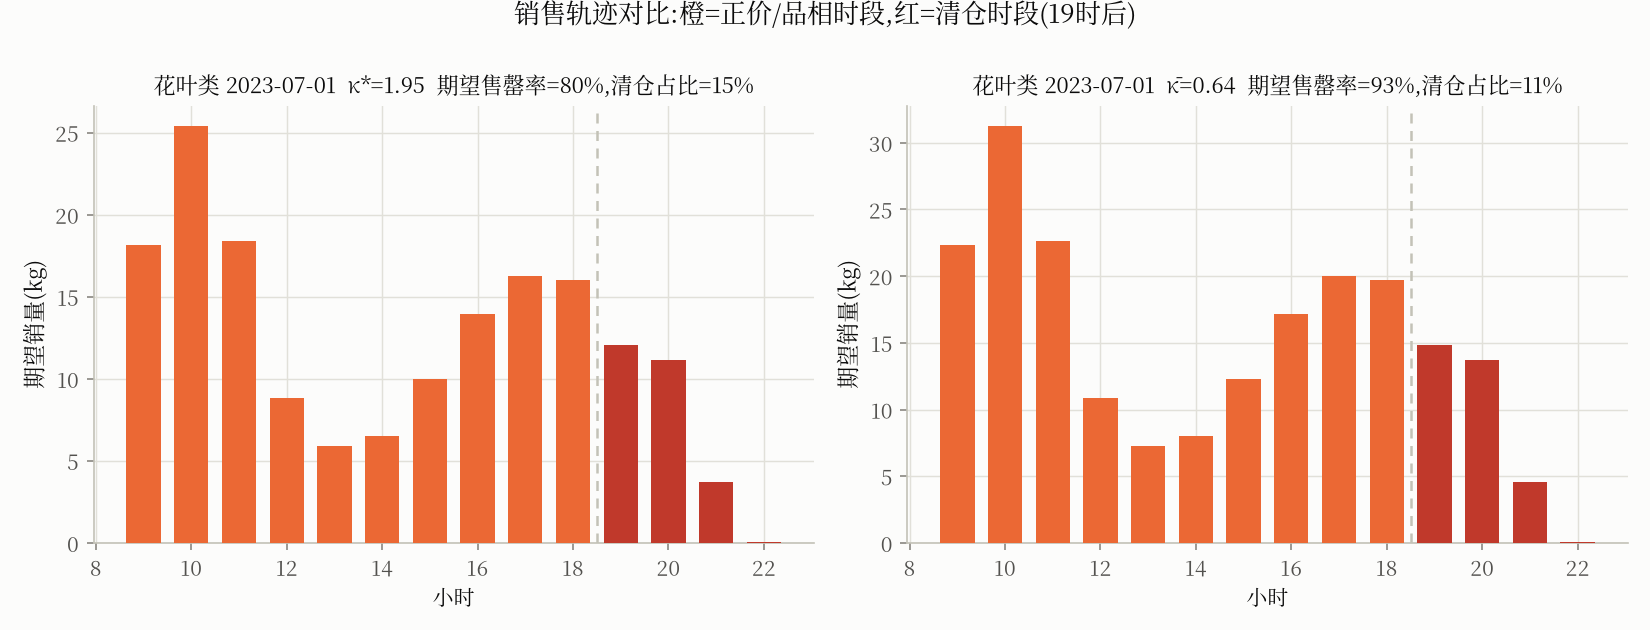
\includegraphics[width=0.92\textwidth]{p2o3_fig2_销售轨迹.png}
  \caption{花叶类 2023 年 7 月 1 日销售轨迹:$\kappa^{\ast}$ 与维持现价 $\bar{\kappa}$ 的对照}
  \label{fig:traj}
\end{figure}

\subsubsection{弹性口径灵敏度与策略区间}

表 \ref{tab:sens} 把三种弹性口径放进同一个优化器,得到的解形态截然不同:数据口径(2SLS 主估计)与后验收缩口径的最优挂牌价全部顶在信任域上缘,而 DML 口径的内点最优恰好落在现价附近,六个品类的平均偏差约 4\%。两个极端把策略空间夹了出来:若数据口径接近真实,应按表 \ref{tab:price} 提价;若 DML 口径接近真实,维持现价已近最优。真实的响应几乎必然介于两者之间,故执行上建议分步上调、逐日监测销量,特别的,一旦实际销量下滑幅度超过半对数模型的预测,即向 DML 口径的内点价回调。失效边界也由此明确:提价建议以响应估计在历史域内成立为前提,域外定价不在模型保护范围之内。

\begin{table}[htbp]
  \centering
  \caption{弹性口径灵敏度:三种口径下的最优挂牌价(2023 年 7 月 1 日,元/kg)}
  \label{tab:sens}
  \begin{tabular}{lccccc}
    \toprule
    品类 & $P^{\ast}$(数据口径) & $P^{\ast}$(后验) & $P^{\ast}$(DML) & 现价 $\bar{P}$ & 解形态 \\
    \midrule
    花叶类 & 10.04(触界) & 10.04(触界) & 5.58(内点) & 5.60 & 提价/维持之争 \\
    食用菌 & 14.63(触界) & 14.63(触界) & 7.95(内点) & 8.23 & 同上 \\
    辣椒类 & 22.39(触界) & 22.39(触界) & 8.50(内点) & 8.43 & 同上 \\
    水生根茎类 & 23.25(触界) & 23.25(触界) & 8.37(内点) & 8.72 & 同上 \\
    茄类 & 16.29(触界) & 16.29(触界) & 9.18(内点) & 8.56 & 同上 \\
    花菜类 & 18.88(触界) & 18.88(触界) & 8.59(内点) & 9.16 & 同上 \\
    \bottomrule
  \end{tabular}
\end{table}

\subsection{定价优化模型评价}

模型的优点有三。其一,需求响应经过了删失修正、工具变量、HAC 标准误与文献先验收缩四重处理,主估计在 5\% 水平显著,且半对数与对数线性两种形式给出的弹性互相印证($-0.12$ 至 $-0.40$ 对 $-0.06$ 至 $-0.43$),结论不依赖单一设定。其二,期望收益直接消费预测分位,预测与定价共享同一套断货时点思想,接口干净,预测的改进会自动传导为定价的改进。其三,一维网格加黄金分割的求解有全局性保证,42 个问题独立可分,结果可复现。

缺点同样具体。其一,品类级销量加权均价含单品构成效应,Laspeyres 对照显示两种口径的系数甚至变号,构成效应的方向无法完全剔除,这是品类级数据的固有限制。其二,删失检测器以 10\% 分位为阈值,轻度断货日(售罄发生在打烊前但晚于 19 时)会被漏检,残留的删失仍使响应估计偏向零。其三,批发价工具变量依赖成本冲击不影响需求的排除性,极端天气同时抬高成本、压低到货质量时,估计仍偏向下界,这解释了我们的弹性为什么低于文献。改进方向是单品级定价实验,哪怕只在两类单品上做两周的价格变动,即可直接识别真实响应,代价是试销期的收益让渡与运营协调成本。

\begin{thebibliography}{9}
% 并入小组主文档时,以下条目移入主文献表并统一编号
\bibitem{ke2017} Ke G, Meng Q, Finley T, et al. LightGBM: A highly efficient gradient boosting decision tree[C]//Advances in Neural Information Processing Systems 30. 2017: 3146-3154.
\bibitem{grinsztajn2022} Grinsztajn L, Oyallon E, Varoquaux G. Why do tree-based models still outperform deep learning on typical tabular data?[C]//Advances in Neural Information Processing Systems 35. 2022.
\bibitem{lyulyov2024} Lyulyov N N. The use of machine learning methods in demand forecasting in retail[C]//IFAC-PapersOnLine, 2024.
\bibitem{fan2024} Fan C L, Kuo C Y, Lu S Y, et al. Optimizing retail demand forecasting with LightGBM for rapid response supply chains[J]. Applied Sciences, 2024, 14(16): 7294.
\bibitem{jain2015} Jain A, Rudi N, Wang T. Demand estimation and ordering under censoring: Stock-out timing is (almost) all you need[J]. Operations Research, 2015, 63(1): 134-150.
\bibitem{phillips2005} Phillips R L. Pricing and Revenue Optimization[M]. Stanford: Stanford University Press, 2005.
\bibitem{besbes2015} Besbes O, Zeevi A. On the (surprising) sufficiency of linear models for optimal pricing[J]. Management Science, 2015, 61(10): 2462-2482.
\bibitem{chernozhukov2018} Chernozhukov V, Chetverikov D, Demirer M, et al. Double/debiased machine learning for treatment and structural parameters[J]. The Econometrics Journal, 2018, 21(1): C1-C68.
\bibitem{andreyeva2010} Andreyeva T, Long M W, Brownell K D. The impact of food prices on consumption: A systematic review of research on the price elasticity of demand for food[J]. American Journal of Public Health, 2010, 100(2): 216-222.
\end{thebibliography}

%%FILL:AI使用声明占位(竞赛要求,参考文献前)%%
